% Generated by pysimcount.figleader -- do not edit; regenerate instead.
% figure: main-t-all-formulas -- mean rank over seeds vs n
% seeds [1, 2, 3, 4, 5, 6, 7, 8, 9, 10]; metric=t kind=xyz merged (Clifford+T (ct), simcount template)
% shown: suzuki4, suzuki6, mo-q6, mo-q14, bm-q10, mo-o8-q21, morales-y8m10, morales-m8
% removed (see main-t-all-formulas-ranking.md): lie-trotter, suzuki2, suzuki8
% rank 1 = cheapest on that seed; equal costs share the mean rank
% per-seed values: runs' totals if measured, else each seed's own fit c(n) ceil(a_s n^b_s)
% derived: main-t-all-formulas.json by pysimcount.figleader; source_sha256=e2b784407e82d3de3175dfa318f56f47f0de675e8adb0038f54747cd6140373b
% figure made at git_commit=eed0c490bd2a7ed3c821acf76ae930c79d2195f6 git_dirty=False
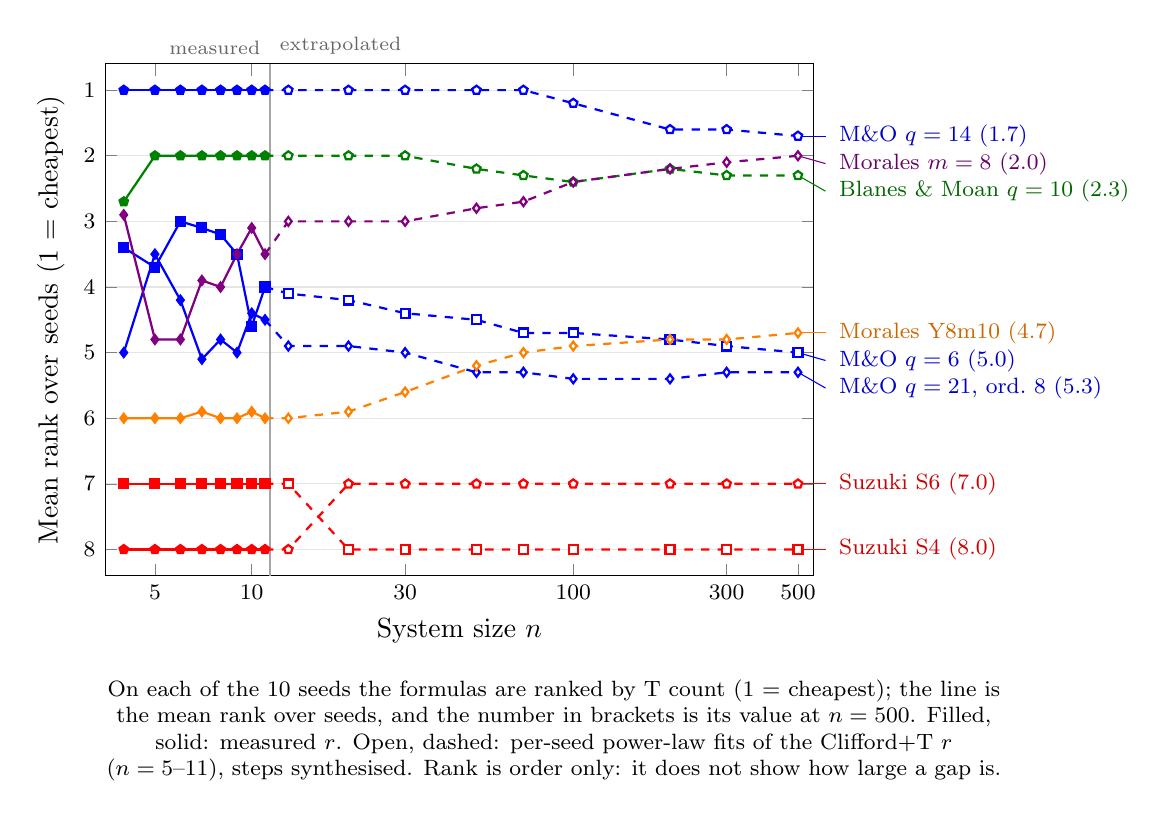
\begin{tikzpicture}
  \begin{semilogxaxis}[
    scale only axis, clip=false,
    width=9.0cm, height=6.5cm,
    xlabel={System size $n$},
    ylabel={Mean rank over seeds (1 = cheapest)},
    xtick={5,10,30,100,300,500}, xticklabels={5,10,30,100,300,500}, xminorticks=false,
    xmin=3.5, xmax=560,
    y dir=reverse, ymin=0.6, ymax=8.4, ytick={1,2,3,4,5,6,7,8},
    ymajorgrids=true, grid style={black!10}, tick label style={font=\footnotesize},
  ]
    \draw[black!35] (axis cs:11.4,0.6) -- (axis cs:11.4,8.4);
    \node[anchor=south east, font=\scriptsize, black!60] at (axis cs:11.4,0.6) {measured};
    \node[anchor=south west, font=\scriptsize, black!60] at (axis cs:11.4,0.6) {extrapolated};
    % suzuki4: mean rank over seeds
    \addplot[red, mark=square*, mark size=1.6pt, line width=0.8pt, solid, mark options={solid, fill=red}] coordinates {
      (4,7)
      (5,7)
      (6,7)
      (7,7)
      (8,7)
      (9,7)
      (10,7)
      (11,7)
    };
    \addplot[red, mark=square*, mark size=1.6pt, line width=0.8pt, dashed, mark options={solid, fill=white}, mark indices={2,...,10}] coordinates {
      (11,7)
      (13,7)
      (20,8)
      (30,8)
      (50,8)
      (70,8)
      (100,8)
      (200,8)
      (300,8)
      (500,8)
    };
    % suzuki6: mean rank over seeds
    \addplot[red, mark=pentagon*, mark size=1.6pt, line width=0.8pt, solid, mark options={solid, fill=red}] coordinates {
      (4,8)
      (5,8)
      (6,8)
      (7,8)
      (8,8)
      (9,8)
      (10,8)
      (11,8)
    };
    \addplot[red, mark=pentagon*, mark size=1.6pt, line width=0.8pt, dashed, mark options={solid, fill=white}, mark indices={2,...,10}] coordinates {
      (11,8)
      (13,8)
      (20,7)
      (30,7)
      (50,7)
      (70,7)
      (100,7)
      (200,7)
      (300,7)
      (500,7)
    };
    % mo-q6: mean rank over seeds
    \addplot[blue, mark=square*, mark size=1.6pt, line width=0.8pt, solid, mark options={solid, fill=blue}] coordinates {
      (4,3.4)
      (5,3.7)
      (6,3)
      (7,3.1)
      (8,3.2)
      (9,3.5)
      (10,4.6)
      (11,4)
    };
    \addplot[blue, mark=square*, mark size=1.6pt, line width=0.8pt, dashed, mark options={solid, fill=white}, mark indices={2,...,10}] coordinates {
      (11,4)
      (13,4.1)
      (20,4.2)
      (30,4.4)
      (50,4.5)
      (70,4.7)
      (100,4.7)
      (200,4.8)
      (300,4.9)
      (500,5)
    };
    % mo-q14: mean rank over seeds
    \addplot[blue, mark=pentagon*, mark size=1.6pt, line width=0.8pt, solid, mark options={solid, fill=blue}] coordinates {
      (4,1)
      (5,1)
      (6,1)
      (7,1)
      (8,1)
      (9,1)
      (10,1)
      (11,1)
    };
    \addplot[blue, mark=pentagon*, mark size=1.6pt, line width=0.8pt, dashed, mark options={solid, fill=white}, mark indices={2,...,10}] coordinates {
      (11,1)
      (13,1)
      (20,1)
      (30,1)
      (50,1)
      (70,1)
      (100,1.2)
      (200,1.6)
      (300,1.6)
      (500,1.7)
    };
    % bm-q10: mean rank over seeds
    \addplot[green!50!black, mark=pentagon*, mark size=1.6pt, line width=0.8pt, solid, mark options={solid, fill=green!50!black}] coordinates {
      (4,2.7)
      (5,2)
      (6,2)
      (7,2)
      (8,2)
      (9,2)
      (10,2)
      (11,2)
    };
    \addplot[green!50!black, mark=pentagon*, mark size=1.6pt, line width=0.8pt, dashed, mark options={solid, fill=white}, mark indices={2,...,10}] coordinates {
      (11,2)
      (13,2)
      (20,2)
      (30,2)
      (50,2.2)
      (70,2.3)
      (100,2.4)
      (200,2.2)
      (300,2.3)
      (500,2.3)
    };
    % mo-o8-q21: mean rank over seeds
    \addplot[blue, mark=diamond*, mark size=1.6pt, line width=0.8pt, solid, mark options={solid, fill=blue}] coordinates {
      (4,5)
      (5,3.5)
      (6,4.2)
      (7,5.1)
      (8,4.8)
      (9,5)
      (10,4.4)
      (11,4.5)
    };
    \addplot[blue, mark=diamond*, mark size=1.6pt, line width=0.8pt, dashed, mark options={solid, fill=white}, mark indices={2,...,10}] coordinates {
      (11,4.5)
      (13,4.9)
      (20,4.9)
      (30,5)
      (50,5.3)
      (70,5.3)
      (100,5.4)
      (200,5.4)
      (300,5.3)
      (500,5.3)
    };
    % morales-y8m10: mean rank over seeds
    \addplot[orange, mark=diamond*, mark size=1.6pt, line width=0.8pt, solid, mark options={solid, fill=orange}] coordinates {
      (4,6)
      (5,6)
      (6,6)
      (7,5.9)
      (8,6)
      (9,6)
      (10,5.9)
      (11,6)
    };
    \addplot[orange, mark=diamond*, mark size=1.6pt, line width=0.8pt, dashed, mark options={solid, fill=white}, mark indices={2,...,10}] coordinates {
      (11,6)
      (13,6)
      (20,5.9)
      (30,5.6)
      (50,5.2)
      (70,5)
      (100,4.9)
      (200,4.8)
      (300,4.8)
      (500,4.7)
    };
    % morales-m8: mean rank over seeds
    \addplot[violet, mark=diamond*, mark size=1.6pt, line width=0.8pt, solid, mark options={solid, fill=violet}] coordinates {
      (4,2.9)
      (5,4.8)
      (6,4.8)
      (7,3.9)
      (8,4)
      (9,3.5)
      (10,3.1)
      (11,3.5)
    };
    \addplot[violet, mark=diamond*, mark size=1.6pt, line width=0.8pt, dashed, mark options={solid, fill=white}, mark indices={2,...,10}] coordinates {
      (11,3.5)
      (13,3)
      (20,3)
      (30,3)
      (50,2.8)
      (70,2.7)
      (100,2.4)
      (200,2.2)
      (300,2.1)
      (500,2)
    };
    \draw[red, line width=0.4pt] (axis cs:500,8) -- ([xshift=0.35cm]axis cs:500,8);
    \node[anchor=west, font=\footnotesize, text=red!80!black] at ([xshift=0.4cm]axis cs:500,8) {Suzuki S4 (8.0)};
    \draw[red, line width=0.4pt] (axis cs:500,7) -- ([xshift=0.35cm]axis cs:500,7);
    \node[anchor=west, font=\footnotesize, text=red!80!black] at ([xshift=0.4cm]axis cs:500,7) {Suzuki S6 (7.0)};
    \draw[blue, line width=0.4pt] (axis cs:500,5) -- ([xshift=0.35cm]axis cs:500,5.12);
    \node[anchor=west, font=\footnotesize, text=blue!80!black] at ([xshift=0.4cm]axis cs:500,5.12) {M\&O $q=6$ (5.0)};
    \draw[blue, line width=0.4pt] (axis cs:500,1.7) -- ([xshift=0.35cm]axis cs:500,1.7);
    \node[anchor=west, font=\footnotesize, text=blue!80!black] at ([xshift=0.4cm]axis cs:500,1.7) {M\&O $q=14$ (1.7)};
    \draw[green!50!black, line width=0.4pt] (axis cs:500,2.3) -- ([xshift=0.35cm]axis cs:500,2.54);
    \node[anchor=west, font=\footnotesize, text=green!50!black!80!black] at ([xshift=0.4cm]axis cs:500,2.54) {Blanes \& Moan $q=10$ (2.3)};
    \draw[blue, line width=0.4pt] (axis cs:500,5.3) -- ([xshift=0.35cm]axis cs:500,5.54);
    \node[anchor=west, font=\footnotesize, text=blue!80!black] at ([xshift=0.4cm]axis cs:500,5.54) {M\&O $q=21$, ord.~8 (5.3)};
    \draw[orange, line width=0.4pt] (axis cs:500,4.7) -- ([xshift=0.35cm]axis cs:500,4.7);
    \node[anchor=west, font=\footnotesize, text=orange!80!black] at ([xshift=0.4cm]axis cs:500,4.7) {Morales Y8m10 (4.7)};
    \draw[violet, line width=0.4pt] (axis cs:500,2) -- ([xshift=0.35cm]axis cs:500,2.12);
    \node[anchor=west, font=\footnotesize, text=violet!80!black] at ([xshift=0.4cm]axis cs:500,2.12) {Morales $m=8$ (2.0)};
  \end{semilogxaxis}
  \node[anchor=north, text width=11.5cm, align=flush center, font=\footnotesize] at (5.7cm,-1.2cm) {On each of the 10 seeds the formulas are ranked by T count (1 = cheapest); the line is the mean rank over seeds, and the number in brackets is its value at $n = 500$. Filled, solid: measured $r$. Open, dashed: per-seed power-law fits of the Clifford+T $r$ ($n = 5$--$11$), steps synthesised. Rank is order only: it does not show how large a gap is.};
\end{tikzpicture}
